\documentclass{article}
\usepackage{graphicx}

\begin{document}

\title{Assignment 1: Design of Experiments\\Mathematics and Statistics, Monsoon 2019}
\author{Jayitha. C\\20171401}

\maketitle


\section{Question 1}
Generate the tables shown in class from the Titanic raw data set.
\begin{enumerate}
  \item Table-I: Economic Status and Sex. Compute (a) population exposed to risk, (b) Number of deaths, and (c) Deaths per 100, exposed to risk, for Male, Female, and Both.
  \item Table-II: Economic Status and Age. Compute (a) population exposed to risk, (b) Number of deaths, and (c) Deaths per 100, exposed to risk, for Adult, Child, and Both.
\end{enumerate}
Write a program in R/C/C++/Python. (submit soft copies of program).
\begin{table}[h!]
  \begin{center}
    \label{tab:table1}
    \begin{tabular}{|c|c|}
      \hline % <-- Toprule here
      \textbf{Column} & \textbf{Variable}\\
      \hline % <-- Midrule here
      1 & Economic Status (0=crew, 1=first, 2 = second, 3 = third)\\
      10 & Age (1 = adult, 0 = child)\\
      19 & Sex (1 = male, 0 = female)\\
      28 & Survived (1 = yes, 0 = no)\\
      \hline % <-- Bottomrule here
    \end{tabular}
  \end{center}
  \caption{Key to Variables in titanic.dat}
\end{table}
\\\\
\textit{\textbf{Answer: }} Refer Figures: \ref{fig:fig1} and \ref{fig:fig2}}

\begin{figure}[h]
  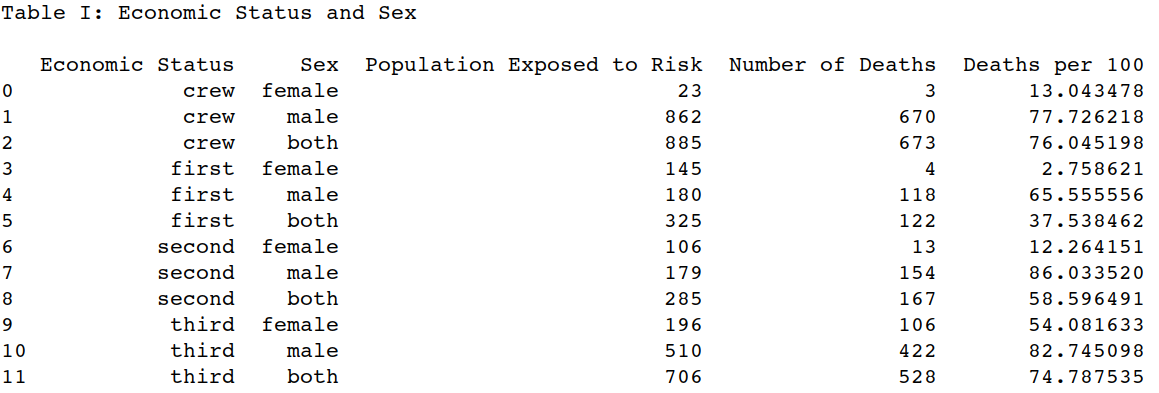
\includegraphics[width=\linewidth]{q1a.png}
  \caption{Economic Status and Sex}
  \label{fig:fig1}
\end{figure}
\begin{figure}[h]
  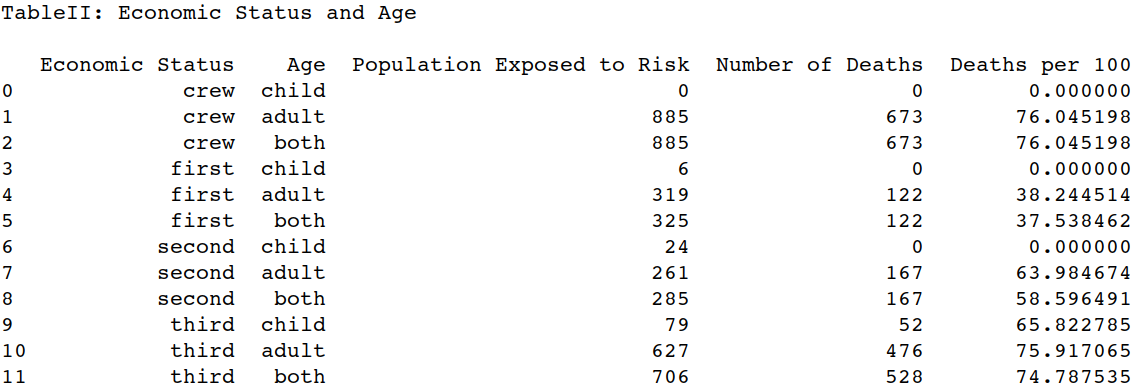
\includegraphics[width=\linewidth]{q1b.png}
  \caption{Economic Status and Age}
  \label{fig:fig2}
\end{figure}
\section{Question 2}
Data from the Salk vaccine field trial suggest that in 1954, the school districts in NFIP trial and in the randomized controlled experiment had similar exposures to the polio virus.

\subsection{Question 2.a}
The data also show that children in the two vaccine groups (for the randomized controlled experiment and the NFIP design) came from families with similar incomes and educational backgrounds. Which two numbers in table confirm this finding?
\\
\\
\textit{\textbf{Answer: }} There are two groups(i.e. two sets of numbers) that suggest that families involved came from similar incomes and educational backgrounds
\\\\
 First, the treatment group of the NFIP experiment consisted of grade 2 children who had familial consent, this would imply that a large part of the group consisted of children from high income families. Similarly, the treatment group of the randomized controlled double-blind experiment consisted of only children who had familial consent, again implying that a large part of the group consisted of children from high income families and backgrounds. As a consequence of this similarity we see that the rates of the treatment classes are 25 and 28 (per 100,000) for the NFIP and the randomized controlled double-blind experiments respectively. These rates are numerically very close.
\\\\
 Second, The no consent groups of both experiments consisted of only children without familial consent and hence a large portion is belived to consist of children from low income families. The rates for these no consent classes are 44 and 46(per 100,000) for the NFIP and randomized controlled double-blind experiments respectively. These numbers are also numerically close.
\\\\
The numbers obtained for the above two groups lead us to believe that the distribution of families and backgrounds involved in the two studies are similar.

\subsection{Question 2.b}
The data show that the children in the no-consent groups had similar family backgrounds. Which pair of numbers in the table confirm this finding?
\\
\\
\textit{\textbf{Answer: }} The no consent group of the NFIP experiment consisted only of grade 2 children without familial consent. This implies that a large portion of this group consisted of children from poor income families. Similarly the no concent group of the randomized controlled double-blind experiment consisted of all children who didn't have familial consent and hence were from poor income families. Therefore the only difference between the groups is that the children from the NFIP experiment group are from grade 2 whereas those of the randomized controlled double-blind experiemnt do not pertain to a single grade. This similarity is so reflected in the numerical closeness of the rates found for the no consent groups. It was 44 and 46(per 100,000) for the NFIP and randomized controlled double-blind experiments respectively.

\subsection{Question 2.c}
The data show that children in the two control groups had different family backgrounds. Which pair of numbers in the table confirm this finding?
\\
\\
\textit{\textbf{Answer: }} The control group of the NFIP experiment consisted of all grade 1 and grade 3 children irrespective of consent, so this group didn't predominantly consist of children from high income families. Whereas the control group of the randomized controlled double-blind experiment consisted of only students with familial consent and therefore a large number of these children were from high income families. To sum up, the two groups are very different where one group consisted of only children with consent(and hence high income family children) and the other had no such filtering criteria. The difference in these two groups is reflected in the rates obtained i.e. 54(per 100,000) for the NFIP experiemnt and 71(per 100,000) for the randomized controlled double-blind experiemnt, which are numerically quite far.

\subsection{Question 2.d}
In the NFIP study, neither the control group nor the no-consent group got the vaccine. Yet the no-consent group had a lower rate of polio. Why?
\\
\\
\textit{\textbf{Answer: }} In the NFIP experiment, the control group consisted of all grade 1 and grade 2 children, this would imply that there was a more or less even distribution of children from both low income and high income families whereas the no consent groups consisted of mostly children from low income families (since it was more likely they couldn't afford the treatment).
\\\\
The paradox pertaining to that time was that it was more likely for a child from a high income family to get polio. Polio is a disease of hygiene children from low income families grow up in borderline unhygienic places, they tend to contract a mild version of polio while still in the mother's womb. Because of this they automatically develop antibodies at a very young age. Whereas children from high income families are brought up in very hygienic places and are more susceptible to contract polio.

\subsection{Question 2.e}
To show that the vaccine works, someone wants to compare the $44/100,000$ in the NFIP study with the $25/100,000$ in the vaccine group. What’s wrong with this idea?
\\
\\
\textit{\textbf{Answer: }} This comparision is biased against the vaccine. The no consent group of grade 2 children predominantly consists of children from low income families and these children are less likely to contract polio. Whereas the treatment group consist of only grade 2 children with familial consent and hence these children are most likely to be from high income families and therefore are more likely to contract polio. The treatment group children are inherently more likely to contract polio when comparent with the no consent group. And hence these numbers aren't a fair representation of the effect of the vaccine in the sense that the vaccine does better than the numbers dipict.

\begin{table}[h]
  \centering
  \begin{tabular}{|c|c|c|}
  \hline
  \textbf{Class}&\textbf{Size}&\textbf{Rate (per 100,000)}\\
  \hline
  Treatment&200,000&28\\
  Control&200,000&71\\
  No consent&350,000&46\\
  \hline
  \end{tabular}
  \caption{Randomized controlled double-blind experiment}
\end{table}

\begin{table}[h]
  \centering
  \begin{tabular}{|c|c|c|}
  \hline
  \textbf{Class}&\textbf{Size}&\textbf{Rate (per 100,000)}\\
  \hline
  Grade 2 (vaccine)&225,000&25\\
Grade 1 \& 3(control)&725,000&54\\
Grade 2 (no consent)&125,000&44\\
  \hline
  \end{tabular}
  \caption{NFIP Study}
\end{table}

\section{Question 3}
From the above tables, those children whose parents refused to participate in the randomized controlled Salk trial got polio at the rate of 46 / 1,00,000. On the other hand, those children whose parents consented to participation got polio at the slightly higher rate of 49 / 1,00,000 in the treatment group and control group taken together. Suppose that this field trial was repeated the following year. On the basis of figures, some parents refused to allow the children to participate in the experiment and be exposed to this higher risk of polio. Were they right? Answer yes or no, and explain briefly.
\\
\\
\textit{\textbf{Answer: }} No, they are not right to refuse the vaccine. If you put the treatment group and control group together, you get a group where all the children had familial consent. And therefore these children are from high income familes. This implies they are implicitly more likely to contract polio.\\\\
Whereas the no consent group consists of children predominantly from low income families and hence they are implicitly less likely to contract polio.
\\\\
These two groups aren't (fairly)comparable since members of one are implicitly more likely to contract than the other. But when comparing the treatment and control groups (which is a fair comparision due to the simmilarity of the groups save the treatment), it shows significant proof of the effectiveness of the vaccine and from a purely precautionary point of view it might be advisable to concede to the vaccine.

\section{Question 4}
What is a randomized controlled double-blind experiment? How is it different from an observational study?
\\
\\
\textit{\textbf{Answer: }} A \textbf{randomized controlled experiment} is one in which to make sure the treatment and control groups are similar, investigators put subjects into any of these two groups at random. A \textbf{double-blind experiemnt} is one in which neither the subjects participating in the study nor those who evaluate their responses know if the subject is in the treatment or control group. A \textbf{randomized controlled double-blind experiment} is one which is both randomized controlled and double-blind.
\\\\
An \textbf{Observation experiemnt} is one in which investigators don't assign subjects into treatment or control groups. Some subjects have conditions which are being studies and they form the treatment group and the rest form the control group. Therefore, in this experiment the subjects assign themselves to the different groups and investigators just study them.

\section{Question 5}
What is confounding factor? Can a confounding factor be controlled in an observational study, if yes, how?
\\
\\
\textit{\textbf{Answer: }} A confounding factor is another variable that the experiment setters haven't accounted for. This variable is associated with the exposure and the disease and accounts for any difference between the control and treatment group other than the treatment itself which is reflected in the responses being studied. \\\\
Although perfect control over confounding factors may not be possible, there does exist the concept of controlling for confounding factors in observational studies. One approach is making comparision in smaller groups, the groups are made smaller and smaller till the control nd treatment groups are similar(homogeneous). This minimises the effect of confounding factors and between two homogeneous groups these factors are non existent.

\section{Question 6}
Define Simpson’s paradox.
\\
\\
\textit{\textbf{Answer: }} \textbf{Simpson's Paradox} is a phenomenon which describes the change of trends that occur when relationships between percentages in subgroups can be reversed when subgroups are combined. For example, comparing relationships between admission rates of men and women department wise and on the whole.




\end{document}
